\section{Tables \& Figures}
\label{sec:tables}

\begin{table}[!h]
    \caption{Country of origin top 10.}
    \label{tab:country-of-origin}

    \begin{subtable}[ht]{.5\textwidth}
    \centering
    \subcaption{Original dataset.}
    \begin{tabular}{cc}
        u.s. & 7330 \\
        unknown & 126 \\
        mexico & 111 \\
        philippines & 60 \\
        de & 50 \\
        puerto rico & 39 \\
        jamaica & 34 \\
        cuba & 34 \\
        el-salvador & 30 \\
        canada & 28 \\
    \end{tabular}
    \end{subtable}
    %
    \begin{subtable}[ht]{.5\textwidth}
    \centering
    \subcaption{New dataset.}
    \begin{tabular}{cc}
        u.s. & 8935 \\
        mexico & 210 \\
        unknown & 185 \\
        philippines & 53 \\
        de & 39 \\
        india & 37 \\
        canada & 32 \\
        gb & 32 \\
        puerto rico & 30 \\
        el-salvador & 29 \\
    \end{tabular}
    \end{subtable}

    \vspace{5mm}

    \begin{subtable}[ht]{.5\textwidth}
    \centering
    \subcaption{New dataset samples with target.}
    \begin{tabular}{cc}
        u.s. & 452 \\
        mexico & 9 \\
        unknown & 8 \\
        de & 4 \\
        india & 3 \\
        hong & 2 \\
        puerto rico & 2 \\
        poland & 2 \\
        china & 2 \\
        ireland & 2 \\
    \end{tabular}
    \end{subtable}
\end{table}


\begin{figure}[!ht]
    \caption{Birth date histograms.}
    \begin{subfigure}[ht]{.5\linewidth}
        \subcaption{Original samples.}
        \label{fig:birth-date-hist-original}
        \centering
        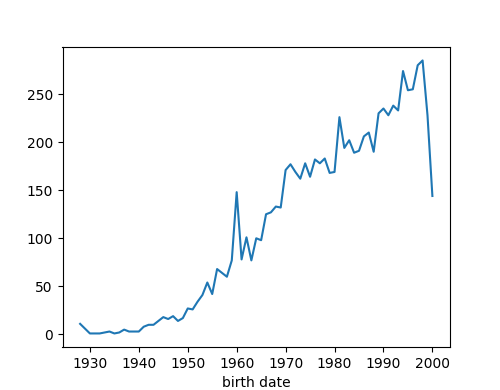
\includegraphics[width=\textwidth]{./img/birth-date-freq-original.png}
    \end{subfigure}
    %
    \begin{subfigure}[ht]{.5\linewidth}
        \subcaption{New samples.}
        \label{fig:birth-date-hist-new}
        \centering
        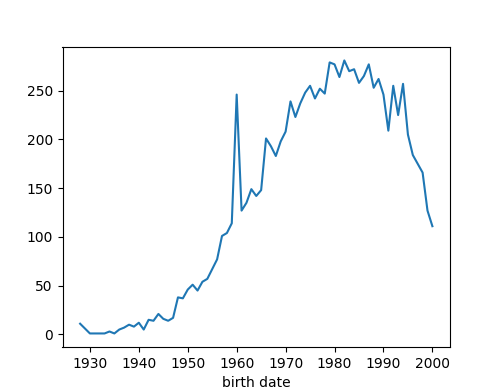
\includegraphics[width=\textwidth]{./img/birth-date-freq-new.png}
    \end{subfigure}

    \vspace{5mm}

    \begin{subfigure}[!ht]{.5\linewidth}
        \subcaption{New samples with outcomes.}
        \label{fig:birth-date-hist-targets}
        \centering
        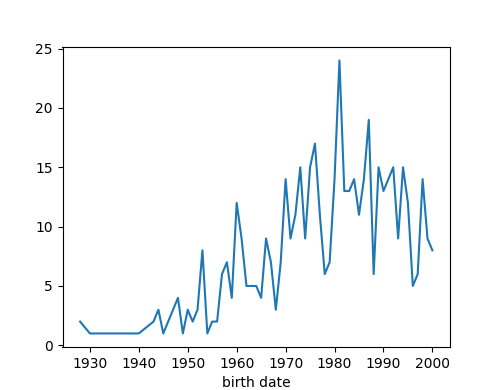
\includegraphics[width=\textwidth]{./img/birth-date-freq-targets.png}
    \end{subfigure}
\end{figure}


\begin{table}[!h]
    \caption{Domestic relationship type value counts.}
    \label{tab:domestic-relationship-type}

    \begin{subtable}[ht]{.5\textwidth}
        \centering
        \subcaption{Original dataset.}
        \begin{tabular}{cc}
            not living with family & 2919 \\
            never married & 2063 \\
            living with child & 1750 \\
            has husband & 1106 \\
            living with extende family & 325 \\
            has wife & 1 \\
        \end{tabular}
    \end{subtable}
    %
    \begin{subtable}[ht]{.5\textwidth}
        \centering
        \subcaption{New dataset.}
        \begin{tabular}{cc}
            has wife & 5398 \\
            not living with family & 2227 \\
            living with child & 1353 \\
            never married & 532 \\
            living with extende family & 245 \\
            has husband & 188 \\
        \end{tabular}
    \end{subtable}

    \vspace{5mm}

    \begin{subtable}[ht]{.5\textwidth}
        \centering
        \subcaption{New dataset samples with target.}
        \begin{tabular}{cc}
            has wife & 266 \\
            not living with family & 119 \\
            living with child & 66 \\
            never married & 23 \\
            living with extende family & 14 \\
            has husband & 10 \\
        \end{tabular}
    \end{subtable}
\end{table}


\begin{table}[!h]
    \caption{Domestic status value counts.}
    \label{tab:domestic-status}

    \begin{subtable}[ht]{.5\textwidth}
        \centering
        \subcaption{Original dataset.}
        \begin{tabular}{cc}
            single & 3662 \\
            d & 2073 \\
            married 2 & 1170 \\
            spouse passed & 599 \\
            divorce pending & 486 \\
            married not together & 163 \\
            married 1 & 11 \\
        \end{tabular}
    \end{subtable}
    %
    \begin{subtable}[ht]{.5\textwidth}
        \centering
        \subcaption{New dataset.}
        \begin{tabular}{cc}
            married 2 & 5645 \\
            single & 2853 \\
            d & 983 \\
            divorce pending & 211 \\
            spouse passed & 154 \\
            married not together & 93 \\
            married 1 & 4 \\
        \end{tabular}
    \end{subtable}

    \vspace{5mm}

    \begin{subtable}[ht]{.5\textwidth}
        \centering
        \subcaption{New dataset samples with target.}
        \begin{tabular}{cc}
            married 2 & 281 \\
            single & 145 \\
            d & 52 \\
            spouse passed & 8 \\
            married not together & 6 \\
            divorce pending & 6 \\
        \end{tabular}
    \end{subtable}
\end{table}


\begin{figure}[!ht]
    \caption{Earned dividends histograms.}
    \label{fig:earned-dividents-hist}

    \begin{subfigure}[ht]{.5\linewidth}
        \subcaption{Original samples.}
        \centering
        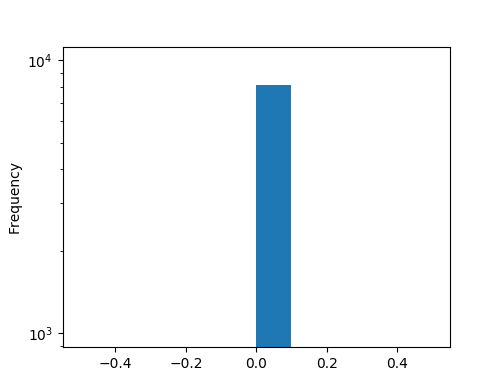
\includegraphics[width=\textwidth]{./img/earned-dividends-hist-original.png}
    \end{subfigure}
    %
    \begin{subfigure}[ht]{.5\linewidth}
        \subcaption{New samples.}
        \centering
        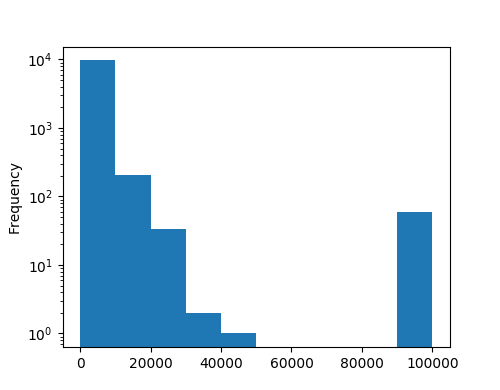
\includegraphics[width=\textwidth]{./img/earned-dividends-hist-new.png}
    \end{subfigure}

    \vspace{5mm}

    \begin{subfigure}[!ht]{.5\linewidth}
        \subcaption{New samples with outcomes.}
        \centering
        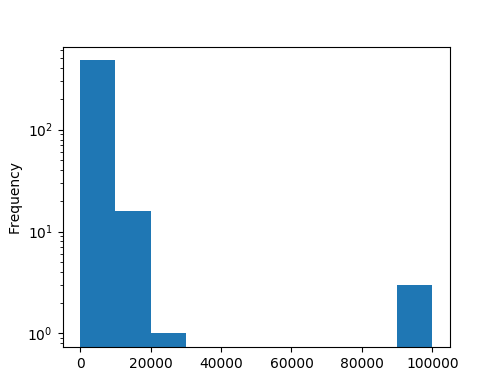
\includegraphics[width=\textwidth]{./img/earned-dividends-hist-targets.png}
    \end{subfigure}
\end{figure}


\begin{table}[!h]
    \caption{Ethnicity value counts.}
    \label{tab:ethnicity}

    \begin{subtable}[ht]{.5\textwidth}
        \centering
        \subcaption{Original dataset.}
        \begin{tabular}{cc}
            white and privileged & 6523 \\
            afro american & 1210 \\
            asian & 262 \\
            american indian & 88 \\
            other & 81 \\
        \end{tabular}
    \end{subtable}
    %
    \begin{subtable}[ht]{.5\textwidth}
        \centering
        \subcaption{New dataset.}
        \begin{tabular}{cc}
            white and privileged & 8679 \\
            afro american & 778 \\
            asian & 315 \\
            american indian & 92 \\
            other & 79 \\
        \end{tabular}
    \end{subtable}

    \vspace{5mm}

    \begin{subtable}[ht]{.5\textwidth}
        \centering
        \subcaption{New dataset samples with target.}
        \begin{tabular}{cc}
            white and privileged & 431 \\
            afro american & 46 \\
            asian & 17 \\
            american indian & 2 \\
            other & 2 \\
        \end{tabular}
    \end{subtable}
\end{table}


\begin{table}[!h]
    \caption{Gender value counts.}
    \label{tab:gender}

    \begin{subtable}[ht]{.5\textwidth}
        \centering
        \subcaption{Original dataset.}
        \begin{tabular}{cc}
            Female & 8164 \\
        \end{tabular}
    \end{subtable}
    %
    \begin{subtable}[ht]{.5\textwidth}
        \centering
        \subcaption{New dataset.}
        \begin{tabular}{cc}
            Male & 8904 \\
            Female & 1039 \\
        \end{tabular}
    \end{subtable}

    \vspace{5mm}

    \begin{subtable}[ht]{.5\textwidth}
        \centering
        \subcaption{New dataset samples with target.}
        \begin{tabular}{cc}
            Male & 453 \\
            Female & 45 \\
        \end{tabular}
    \end{subtable}
\end{table}


\begin{table}[!h]
    \caption{Job type value counts.}
    \label{tab:job-type}

    \begin{subtable}[ht]{.5\textwidth}
        \centering
        \subcaption{Original dataset.}
        \begin{tabular}{cc}
            private & 5919 \\
            unknown & 620 \\
            local-gov & 618 \\
            state-gov & 368 \\
            self-emp-not-inc & 303 \\
            federal-gov & 236 \\
            self-emp-inc & 94 \\
            without-pay & 4 \\
            never-worked & 2 \\
        \end{tabular}
    \end{subtable}
    %
    \begin{subtable}[ht]{.5\textwidth}
        \centering
        \subcaption{New dataset.}
        \begin{tabular}{cc}
            private & 6824 \\
            self-emp-not-inc & 905 \\
            local-gov & 573 \\
            unknown & 489 \\
            self-emp-inc & 426 \\
            state-gov & 415 \\
            federal-gov & 304 \\
            without-pay & 4 \\
            never-worked & 3 \\
        \end{tabular}
    \end{subtable}

    \vspace{5mm}

    \begin{subtable}[ht]{.5\textwidth}
        \centering
        \subcaption{New dataset samples with target.}
        \begin{tabular}{cc}
            private & 341 \\
            self-emp-not-inc & 44 \\
            unknown & 28 \\
            local-gov & 28 \\
            self-emp-inc & 24 \\
            state-gov & 20 \\
            federal-gov & 13 \\
        \end{tabular}
    \end{subtable}
\end{table}


\begin{figure}[!ht]
    \caption{Interest earned histograms.}
    \label{fig:interest-earned-hist}

    \begin{subfigure}[ht]{.5\linewidth}
        \subcaption{Original samples.}
        \centering
        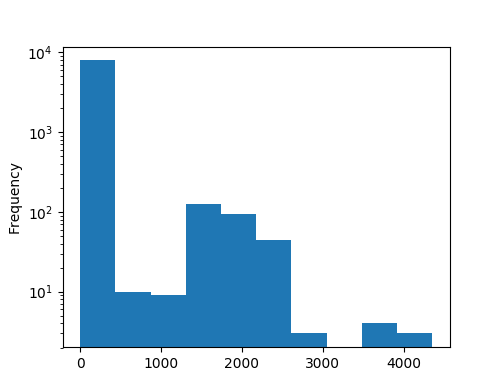
\includegraphics[width=\textwidth]{./img/interest-earned-original.png}
    \end{subfigure}
    %
    \begin{subfigure}[ht]{.5\linewidth}
        \subcaption{New samples.}
        \centering
        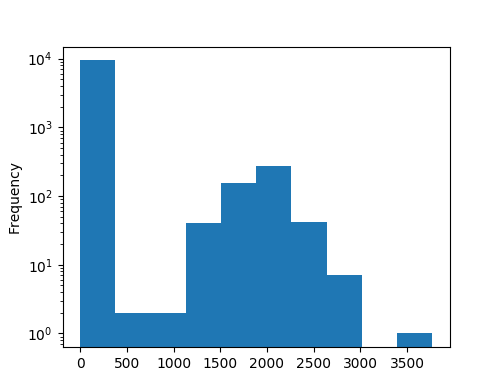
\includegraphics[width=\textwidth]{./img/interest-earned-new.png}
    \end{subfigure}

    \vspace{5mm}

    \begin{subfigure}[!ht]{.5\linewidth}
        \subcaption{New samples with outcomes.}
        \centering
        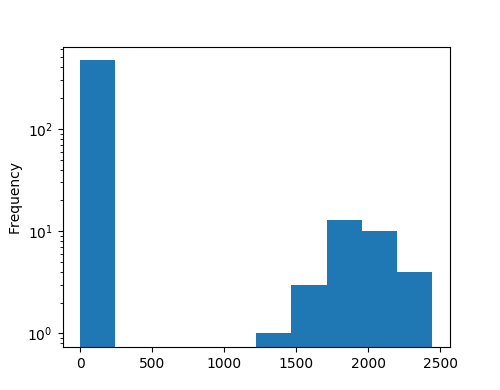
\includegraphics[width=\textwidth]{./img/interest-earned-targets.png}
    \end{subfigure}
\end{figure}


\begin{figure}[!ht]
    \caption{Monthly work histograms.}
    \label{fig:monthly-work-hist}

    \begin{subfigure}[ht]{.5\linewidth}
        \subcaption{Original samples.}
        \centering
        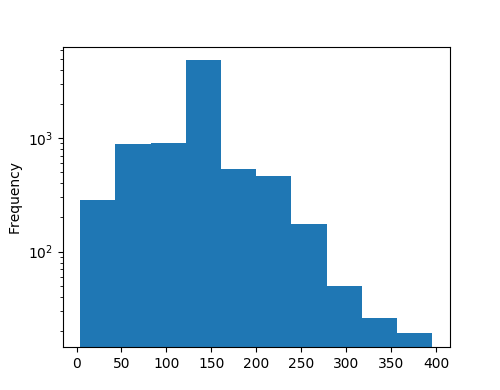
\includegraphics[width=\textwidth]{./img/monthly-work-original.png}
    \end{subfigure}
    %
    \begin{subfigure}[ht]{.5\linewidth}
        \subcaption{New samples.}
        \centering
        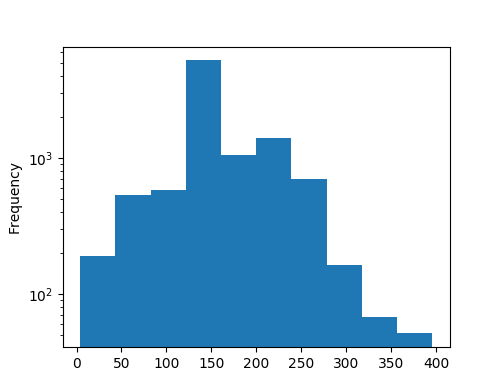
\includegraphics[width=\textwidth]{./img/monthly-work-new.png}
    \end{subfigure}

    \vspace{5mm}

    \begin{subfigure}[!ht]{.5\linewidth}
        \subcaption{New samples with outcomes.}
        \centering
        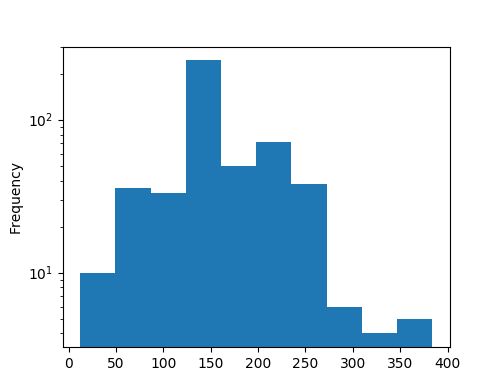
\includegraphics[width=\textwidth]{./img/monthly-work-targets.png}
    \end{subfigure}
\end{figure}


\begin{table}[!h]
    \caption{Profession value counts.}
    \label{tab:profession}

    \begin{subtable}[ht]{.5\textwidth}
        \centering
        \subcaption{Original dataset.}
        \begin{tabular}{cc}
            secretarial & 1949 \\
            other & 1423 \\
            specialist technician & 1096 \\
            sales & 978 \\
            C-level & 842 \\
            unknown & 622 \\
            mechanic & 420 \\
            technology support & 247 \\
            vocational & 184 \\
            household labor & 131 \\
            estate employee & 108 \\
            defense contractor & 58 \\
            trucking & 58 \\
            agriculture & 48 \\
        \end{tabular}
    \end{subtable}
    %
    \begin{subtable}[ht]{.5\textwidth}
        \centering
        \subcaption{New dataset.}
        \begin{tabular}{cc}
            vocational & 1561 \\
            C-level & 1316 \\
            specialist technician & 1213 \\
            sales & 1112 \\
            other & 780 \\
            secretarial & 736 \\
            trucking & 666 \\
            mechanic & 637 \\
            household labor & 501 \\
            unknown & 492 \\
            agriculture & 388 \\
            technology support & 279 \\
            defense contractor & 244 \\
            estate employee & 16 \\
            army & 2 \\
        \end{tabular}
    \end{subtable}

    \vspace{5mm}

    \begin{subtable}[ht]{.5\textwidth}
        \centering
        \subcaption{New dataset samples with target.}
        \begin{tabular}{cc}
            C-level & 68 \\
            vocational & 68 \\
            sales & 64 \\
            specialist technician & 49 \\
            other & 42 \\
            trucking & 38 \\
            household labor & 33 \\
            mechanic & 30 \\
            secretarial & 29 \\
            unknown & 28 \\
            defense contractor & 18 \\
            agriculture & 17 \\
            technology support & 13 \\
            army & 1 \\
        \end{tabular}
    \end{subtable}
\end{table}


\begin{table}[!h]
    \caption{School level value counts.}
    \label{tab:}

    \begin{subtable}[ht]{.5\textwidth}
        \centering
        \subcaption{Original dataset.}
        \begin{tabular}{cc}
            secondary & 2594 \\
            entry level college & 2165 \\
            college graduate & 1188 \\
            basic vocational & 373 \\
            some post graduate & 355 \\
            secondary 11 & 341 \\
            advanced vocational & 326 \\
            10th & 248 \\
            secondary-7 through 8 & 123 \\
            secondary 12 & 106 \\
            secondary-9 & 104 \\
            secondary-5 through 6 & 72 \\
            advanced post graduate & 61 \\
            primary school & 58 \\
            primary 1 through 4 & 37 \\
            kindergarten & 13 \\
        \end{tabular}
    \end{subtable}
    %
    \begin{subtable}[ht]{.5\textwidth}
        \centering
        \subcaption{New dataset.}
        \begin{tabular}{cc}
            secondary & 3243 \\
            entry level college & 2087 \\
            college graduate & 1691 \\
            some post graduate & 577 \\
            basic vocational & 402 \\
            secondary 11 & 317 \\
            advanced vocational & 303 \\
            10th & 277 \\
            secondary-7 through 8 & 208 \\
            primary school & 202 \\
            secondary-9 & 172 \\
            advanced post graduate & 142 \\
            secondary 12 & 140 \\
            secondary-5 through 6 & 117 \\
            primary 1 through 4 & 49 \\
            kindergarten & 16 \\
        \end{tabular}
    \end{subtable}

    \vspace{5mm}

    \begin{subtable}[ht]{.5\textwidth}
        \centering
        \subcaption{New dataset samples with target.}
        \begin{tabular}{cc}
            secondary & 179 \\
            entry level college & 110 \\
            college graduate & 76 \\
            some post graduate & 26 \\
            secondary 11 & 20 \\
            primary school & 13 \\
            10th & 12 \\
            advanced vocational & 11 \\
            secondary 12 & 10 \\
            secondary-9 & 9 \\
            basic vocational & 9 \\
            advanced post graduate & 8 \\
            secondary-5 through 6 & 5 \\
            secondary-7 through 8 & 5 \\
            kindergarten & 3 \\
            primary 1 through 4 & 2 \\
        \end{tabular}
    \end{subtable}
\end{table}
